\chapter{METODOLOGI PENELITIAN}

\section{Waktu, Tempat, dan Jadwal Penelitian}

\subsection{Waktu Pelaksanaan Penelitian}
Penelitian ini dilaksanakan selama lima bulan, dimulai dari bulan \textbf{[BULAN AWAL TAHUN]} hingga \textbf{[BULAN AKHIR TAHUN]}. Keseluruhan proses penelitian mencakup enam tahapan utama yang dilaksanakan secara berurutan dan iteratif, yaitu studi literatur, analisis sistem eksisting, pengumpulan dan preprocessing data, pengembangan model kecerdasan buatan, implementasi sistem, serta pengujian dan evaluasi performa.

\subsection{Tempat Pelaksanaan Penelitian}
Penelitian ini dilaksanakan di PT Lare Osing Ndo yang berlokasi di \textbf{[ALAMAT LENGKAP PERUSAHAAN, KOTA, KODE POS]}. Pengambilan data primer dilakukan secara langsung pada infrastruktur jaringan perusahaan yang terdiri dari \textbf{[JUMLAH]} perangkat aktif dengan kombinasi router dan switch dari vendor Juniper, Huawei, dan MikroTik. Proses pengembangan sistem dilakukan menggunakan workstation portabel Lenovo ThinkPad T14 Gen 4, sementara proses pelatihan model dilakukan pada lingkungan komputasi lokal dengan spesifikasi yang mendukung operasi pembelajaran mesin.

\subsection{Jadwal Penelitian}
Jadwal kegiatan penelitian dirancang secara iteratif mengingat sifat pengembangan sistem berbasis kecerdasan buatan yang memerlukan siklus pengujian dan penyempurnaan berulang. Rincian lengkap jadwal penelitian disajikan pada Tabel \ref{tab:jadwal_penelitian}.

\begin{table}[H]
    \centering
    \caption{Jadwal Kegiatan Penelitian}
    \label{tab:jadwal_penelitian}
    \begin{tabular}{|c|l|c|c|c|c|c|}
        \hline
        \textbf{No} & \textbf{Kegiatan} & \textbf{Bulan 1} & \textbf{Bulan 2} & \textbf{Bulan 3} & \textbf{Bulan 4} & \textbf{Bulan 5} \\ \hline
        1 & Studi Literatur & \checkmark & & & & \\ \hline
        2 & Analisis Sistem Eksisting & \checkmark & \checkmark & & & \\ \hline
        3 & Pengumpulan Data & & \checkmark & \checkmark & & \\ \hline
        4 & Preprocessing \& Pelabelan & & & \checkmark & & \\ \hline
        5 & Pengembangan Model AI & & & \checkmark & \checkmark & \\ \hline
        6 & Implementasi Sistem & & & & \checkmark & \checkmark \\ \hline
        7 & Pengujian \& Evaluasi & & & & & \checkmark \\ \hline
        8 & Penyusunan Laporan & & & & \checkmark & \checkmark \\ \hline
    \end{tabular}
\end{table}

\section{Alat dan Bahan Penelitian}

Penelitian ini memerlukan kombinasi perangkat keras dan perangkat lunak khusus untuk mendukung pengembangan sistem berbasis pembelajaran mesin pada jaringan komputer.

\subsection{Perangkat Keras (\textit{Hardware})}

Workstation development yang digunakan adalah Lenovo ThinkPad T14 Gen 4 dengan prosesor Intel Core i7-1370P generasi ke-13 yang memiliki 20 logical cores, dilengkapi dengan Intel Iris Xe Graphics (RPL-P) dan memori sebesar 32 GB RAM. Sistem operasi yang digunakan adalah Fedora Linux 43 (Workstation Edition) dengan kernel versi 6.17.12 dan windowing system Wayland. Workstation ini digunakan untuk seluruh proses pengembangan, mulai dari pemrograman backend, pengembangan model AI, hingga deployment sistem.

Perangkat jaringan fisik yang menjadi objek penelitian terdiri dari router dan switch dari tiga vendor berbeda, yaitu Juniper dengan sistem operasi JunOS, Huawei dengan VRP Operating System, dan MikroTik dengan RouterOS. Perangkat-perangkat ini merupakan infrastruktur jaringan aktif PT Lare Osing Ndo yang menjadi objek monitoring dan sumber data penelitian.

\subsection{Perangkat Lunak (\textit{Software})}

Pengembangan backend sistem menggunakan Bun sebagai JavaScript/TypeScript runtime yang dioptimasi untuk performa tinggi, dengan Hono sebagai lightweight web framework. Untuk penyimpanan data time-series digunakan PostgreSQL yang dikelola melalui Drizzle ORM, sedangkan polling data dari perangkat jaringan menggunakan library Net-SNMP.

Stack pengembangan machine learning menggunakan Python versi 3.x sebagai bahasa pemrograman utama. Framework deep learning yang digunakan adalah PyTorch dengan PyTorch Geometric sebagai library khusus untuk Graph Neural Network. Untuk menyediakan ML inference service digunakan FastAPI, sementara manipulasi data numerik menggunakan NumPy dan Pandas. Analisis graf dilakukan menggunakan NetworkX, dan visualisasi hasil training menggunakan Matplotlib.

Supporting tools yang digunakan meliputi Docker untuk kontainerisasi aplikasi, Git untuk version control, serta data export/import tools yang terintegrasi dalam sistem frontend.

\subsection{Bahan Penelitian}

Data primer dikumpulkan secara real-time melalui protokol SNMP dengan interval polling setiap 1 menit. Data ini mencakup metrik performa node seperti CPU usage, RAM usage, total traffic in/out, interface utilization, dan status operasional perangkat. Untuk level link, data yang dikumpulkan meliputi link quality, bandwidth utilization, interface speed, jarak fisik antar node, dan status koneksi. Selain itu, dikumpulkan juga data konfigurasi VLAN dan topologi jaringan layer 2.

Data sekunder diperoleh dari hasil kuesioner pakar untuk pembobotan kriteria menggunakan metode Analytic Hierarchy Process (AHP), serta dokumentasi arsitektur jaringan eksisting PT Lare Osing Ndo.

\section{Gambaran Umum Sistem}

\subsection{Sistem Saat Ini (\textit{Current State})}

Infrastruktur jaringan PT Lare Osing Ndo saat ini menggunakan topologi hybrid dengan kombinasi perangkat dari berbagai vendor, yaitu Juniper, Huawei, dan MikroTik. Manajemen lalu lintas data pada layer 2 dilakukan melalui konfigurasi routing VLAN secara manual oleh network engineer. Dalam pendekatan ini, administrator menentukan secara eksplisit jalur yang akan dilalui oleh setiap VLAN untuk mencapai client, dengan tujuan memanfaatkan multiple link redundan yang telah dibangun.

Strategi manual ini memberikan fleksibilitas dalam distribusi trafik antar jalur dan memungkinkan utilisasi bandwidth yang lebih optimal dibandingkan hanya menggunakan satu jalur aktif. Namun, pendekatan ini menimbulkan sejumlah kendala operasional yang signifikan. Risiko looping sangat tinggi karena tanpa mekanisme loop prevention otomatis, kesalahan konfigurasi dapat menyebabkan broadcast storm yang melumpuhkan seluruh segmen jaringan. Kompleksitas manajemen meningkat seiring bertambahnya jumlah VLAN dan link redundan, dimana pemetaan manual jalur untuk setiap VLAN menjadi semakin rumit dan dokumentasi routing path sulit dijaga konsistensinya.

Keputusan routing yang berbasis intuisi dan pengalaman administrator tidak selalu menghasilkan distribusi trafik yang optimal. Beberapa link sering mengalami kongesti sementara link lainnya tidak termanfaatkan dengan baik, mengakibatkan pemborosan sumber daya infrastruktur. Ketika terjadi kegagalan link atau degradasi performa perangkat, proses reconfiguration manual memerlukan waktu yang signifikan karena administrator harus mengidentifikasi masalah, menganalisis jalur alternatif yang tersedia, merencanakan konfigurasi baru, dan menerapkannya ke perangkat-perangkat terkait.

Sistem saat ini bersifat reaktif dan tidak memiliki mekanisme prediktif untuk mengantisipasi degradasi performa atau kegagalan link berdasarkan analisis pola trafik historis. Administrator juga tidak memiliki dashboard terpusat yang menampilkan kondisi kesehatan jaringan secara menyeluruh, sehingga monitoring dilakukan secara parsial pada masing-masing perangkat. Konfigurasi manual yang dilakukan berulang kali pada puluhan perangkat dengan vendor dan sintaks yang berbeda-beda sangat rentan terhadap human error, terutama pada kondisi darurat atau saat administrator bekerja di bawah tekanan untuk memulihkan layanan dengan cepat.

Kondisi ini mengakibatkan overhead operasional yang tinggi, meningkatkan risiko downtime, dan berpotensi melanggar Service Level Agreement (SLA) yang telah ditetapkan kepada pelanggan. Oleh karena itu, diperlukan sistem cerdas yang dapat memberikan rekomendasi jalur optimal secara otomatis dengan mempertimbangkan berbagai metrik performa jaringan secara real-time, sekaligus meminimalkan risiko looping dan human error dalam proses konfigurasi.

\subsection{Sistem yang Diusulkan (\textit{Proposed System})}
Penelitian ini mengusulkan sistem cerdas bernama "Laros Watch" yang mengintegrasikan Network Management System (NMS) berbasis SNMP dengan mesin kecerdasan buatan berbasis Graph Attention Network (GAT). Sistem ini dirancang untuk memberikan rekomendasi jalur optimal secara real-time dengan mempertimbangkan berbagai metrik performa jaringan secara holistik. Arsitektur sistem yang diusulkan divisualisasikan pada Gambar \ref{fig:arsitektur_sistem}.

\begin{figure}[H]
    \centering
    \includegraphics[width=0.95\textwidth]{images/laros_watch_infra.png}
    \caption{Arsitektur Sistem Laros Watch (Proposed Architecture)}
    \label{fig:arsitektur_sistem}
\end{figure}

Arsitektur sistem terdiri dari empat layer utama yang bekerja secara terintegrasi. Physical Network Layer merupakan infrastruktur jaringan fisik tempat perangkat router dan switch beroperasi, dimana perangkat-perangkat dari vendor Juniper, Huawei, dan MikroTik saling terkoneksi membentuk topologi hybrid. Setiap perangkat dikonfigurasi dengan SNMP agent yang memungkinkan sistem melakukan polling data secara periodik.

Data Collection \& Storage Layer bertanggung jawab untuk pengumpulan dan penyimpanan data monitoring. Backend service melakukan polling SNMP ke setiap perangkat setiap 1 menit untuk mengambil data real-time. Sistem mendukung Object Identifier (OID) yang berbeda untuk setiap vendor dan melakukan normalisasi data ke range [0,1] untuk memudahkan processing oleh model AI. Seluruh data disimpan dalam PostgreSQL dengan struktur yang dioptimasi untuk query time-series.

Core Backend (Application Layer) dibangun menggunakan Bun runtime dan Hono framework dengan arsitektur modular. Layer ini mengelola berbagai service seperti SNMP Poller Service untuk proses polling data dari perangkat jaringan, Device Discovery Service untuk auto-discovery perangkat baru, VLAN Configuration Service untuk mengelola data konfigurasi VLAN, Data Aggregation Service untuk mengagregasi data dari berbagai sumber, API Gateway untuk menyediakan RESTful API, dan Database Layer menggunakan Drizzle ORM untuk manajemen koneksi database.

ML Engine (Intelligence Layer) merupakan inti dari sistem kecerdasan buatan yang dibangun menggunakan Python dengan FastAPI sebagai service wrapper. Layer ini terdiri dari Graph Construction Module untuk mengkonversi data jaringan menjadi representasi graf, Feature Engineering Module untuk memproses fitur-fitur node dan edge, GAT Inference Engine untuk menghasilkan node embeddings, Path Recommendation Module untuk menghitung skor kualitas jalur dan memberikan Top-K rekomendasi, serta AHP Weighting Module untuk menerapkan bobot preferensi dari hasil kuesioner pakar.

Presentation Layer (Frontend) merupakan antarmuka pengguna yang menampilkan visualisasi topologi jaringan, status real-time perangkat, rekomendasi jalur optimal, serta menyediakan fitur export data untuk keperluan re-training model.

\subsection{Alur Kerja Sistem}
Sistem Laros Watch beroperasi melalui alur kerja yang terintegrasi antara komponen monitoring, kecerdasan buatan, dan antarmuka pengguna. Untuk mempermudah pemahaman, alur kerja sistem divisualisasikan dalam bentuk diagram alir pada Gambar~\ref{fig:system_workflow}.

\begin{figure}[htbp]
    \centering
    \begin{tikzpicture}[
        node distance=1.2cm,
        box/.style={rectangle, draw, minimum width=3.5cm, minimum height=1cm, align=center, font=\small},
        decision/.style={diamond, draw, minimum width=3cm, minimum height=1cm, align=center, font=\small, aspect=2},
        arrow/.style={->, >=stealth, thick}
    ]

    \node[box] (snmp) {SNMP Polling\\(setiap 1 menit)};
    \node[box, below=of snmp] (db) {Simpan ke PostgreSQL};
    \node[decision, below=of db] (trigger) {Perubahan Status\\atau User Request?};
    \node[box, below=of trigger] (api) {Kirim Snapshot\\ke ML Engine (REST API)};
    \node[box, below=of api] (graph) {Konversi ke\\PyTorch Geometric Graph};
    \node[box, below=of graph] (gat) {GAT Inference\\(Node Embeddings)};
    \node[box, below=of gat] (score) {Path Scoring\\(Quality Computation)};
    \node[box, below=of score] (topk) {Return Top-K\\Best Paths};
    \node[box, below=of topk] (ui) {Visualisasi di Frontend};
    \node[box, below=of ui] (admin) {Administrator\\Decision \& Configuration};

    \draw[arrow] (snmp) -- (db);
    \draw[arrow] (db) -- (trigger);
    \draw[arrow] (trigger) -- node[right] {Ya} (api);
    \draw[arrow] (trigger.east) -- ++(2,0) node[right] {Tidak} |- (snmp.east);
    \draw[arrow] (api) -- (graph);
    \draw[arrow] (graph) -- (gat);
    \draw[arrow] (gat) -- (score);
    \draw[arrow] (score) -- (topk);
    \draw[arrow] (topk) -- (ui);
    \draw[arrow] (ui) -- (admin);
    \draw[arrow] (admin.west) -- ++(-2,0) |- (snmp.west);

    \end{tikzpicture}
    \caption{Diagram Alur Kerja Sistem Laros Watch}
    \label{fig:system_workflow}
\end{figure}

Proses dimulai dengan tahap data collection dimana backend service melakukan polling SNMP ke seluruh perangkat jaringan secara periodik dengan interval 1 menit. Data yang dikumpulkan mencakup metrik node seperti CPU usage, RAM usage, total traffic in/out, interface utilization, dan operational status, serta metrik edge seperti link quality, bandwidth utilization bidirectional, interface speed, distance, dan link status. Selain itu, dikumpulkan juga konfigurasi VLAN meliputi VLAN membership, tagged/untagged ports, dan topologi logical.

Seluruh data hasil polling disimpan ke database PostgreSQL dengan struktur time-series yang dioptimasi untuk query performa historis. Database ini berfungsi sebagai historical repository untuk menyimpan riwayat performa jaringan, real-time cache untuk menyediakan akses cepat ke data terkini, dan training data source untuk re-training model secara berkala.

Proses inferensi model AI dapat dipicu oleh dua kondisi, yaitu event-driven ketika sistem mendeteksi perubahan signifikan pada status node atau link (seperti link down, CPU usage lebih dari 80\%, atau bandwidth utilization lebih dari 90\%), atau user-requested ketika network administrator secara eksplisit meminta rekomendasi jalur optimal melalui frontend interface. Ketika salah satu kondisi terpenuhi, backend mengambil snapshot data terkini dari database dan mengirimkannya ke ML Engine melalui REST API.

ML Engine menerima data snapshot dan melakukan transformasi menjadi struktur graf yang sesuai dengan format PyTorch Geometric. Setiap perangkat jaringan direpresentasikan sebagai node dengan feature vector $\mathbf{h}_i \in \mathbb{R}^6$, setiap koneksi antar perangkat direpresentasikan sebagai edge dengan feature vector $\mathbf{e}_{ij} \in \mathbb{R}^7$, dan struktur topologi jaringan direpresentasikan dalam bentuk adjacency list untuk efisiensi komputasi.

Model Graph Attention Network yang telah terlatih melakukan forward pass untuk menghasilkan node embeddings $\mathbf{h}'_i \in \mathbb{R}^{64}$. Proses ini melibatkan perhitungan attention coefficients $\alpha_{ij}$ untuk setiap pasangan node yang terhubung, agregasi informasi dari node tetangga dengan bobot sesuai attention coefficients, dan pemrosesan melalui 3 layer GAT untuk menangkap pola kompleks dalam radius 3-hop neighborhood.

Algoritma path recommendation kemudian menghitung skor kualitas untuk semua jalur yang mungkin antara source dan target node. Proses ini mencakup path enumeration untuk generate semua jalur valid dengan dynamic cutoff, quality computation untuk setiap jalur menggunakan Path Quality Predictor (MLP), penerapan hop penalty untuk jalur dengan jumlah hop yang lebih panjang, dan ranking jalur berdasarkan skor kualitas secara descending.

Top-K jalur terbaik (default K=5) beserta skor kualitas masing-masing dikembalikan ke backend melalui response API. Hasil ini mencakup path sequence berupa urutan node yang dilalui, quality score dalam range [0, 1] dengan interpretasi nilai lebih dari 0.8 sebagai excellent, 0.6-0.8 sebagai good, 0.4-0.6 sebagai fair, dan kurang dari 0.4 sebagai poor, serta metrics summary berupa agregat metrik untuk setiap jalur.

Frontend menampilkan hasil rekomendasi kepada network administrator dalam bentuk interactive topology graph dengan highlighting pada jalur rekomendasi, comparison table untuk perbandingan metrik Top-K jalur, dan historical trend berupa grafik trend performa untuk jalur yang dipilih. Administrator dapat menggunakan informasi ini untuk menerapkan konfigurasi VLAN routing secara manual atau membandingkan rekomendasi sistem dengan intuisi expert untuk validasi keputusan. Setelah keputusan routing diterapkan, sistem kembali melanjutkan monitoring kontinyu dimana perubahan kondisi jaringan akan memicu inferensi ulang secara otomatis, menciptakan siklus continuous improvement.

\section{Tahapan Penelitian}
Penelitian ini dirancang mengikuti metodologi penelitian kuantitatif dengan pendekatan eksperimental. Alur penelitian secara umum mengikuti kerangka kerja Machine Learning Development Lifecycle yang divisualisasikan pada Gambar \ref{fig:alur_penelitian}.

\begin{figure}[H]
    \centering
    \includegraphics[width=0.5\textwidth]{images/flowchart3.png}
    \caption{Diagram Alur Metodologi Penelitian}
    \label{fig:alur_penelitian}
\end{figure}

\subsection{Identifikasi Masalah dan Studi Literatur}
Tahap awal penelitian dimulai dengan identifikasi masalah pada sistem manajemen jaringan eksisting PT Lare Osing Ndo. Permasalahan utama yang teridentifikasi adalah keterbatasan pendekatan manual routing VLAN dalam menangani distribusi beban dan adaptasi terhadap perubahan kondisi jaringan secara dinamis, serta tingginya risiko looping dan human error.

Studi literatur dilakukan untuk mengkaji state-of-the-art dalam intelligent network management, aplikasi Graph Neural Networks untuk optimasi routing, metode multi-criteria decision making seperti AHP, protokol monitoring jaringan seperti SNMP, NetFlow, dan sFlow, serta best practices dalam implementasi sistem NMS. Hasil studi literatur menjadi landasan teoritis dalam perancangan arsitektur sistem dan pemilihan metode yang sesuai.

\subsection{Perancangan Arsitektur Sistem}

Berdasarkan hasil analisis masalah dan studi literatur, dirancang arsitektur sistem Laros Watch yang mempertimbangkan aspek skalabilitas, \textit{maintainability}, dan integrasi dengan infrastruktur eksisting. Perancangan ini mencakup definisi struktur graf untuk representasi topologi jaringan serta arsitektur model GAT yang sesuai dengan karakteristik data. Detail perancangan fungsional dan basis data dijabarkan pada sub-bab berikut.

\subsubsection{Perancangan Fungsional Sistem (Use Case Diagram)}
Perancangan fungsionalitas sistem dimodelkan menggunakan \textit{Use Case Diagram} untuk mendefinisikan interaksi antara pengguna dan sistem Laros Watch. Rancangan ini mencakup definisi aktor yang terlibat serta alur proses utama, mulai dari mekanisme \textit{polling} data, manajemen perangkat, hingga visualisasi hasil prediksi anomali. Diagram ini menjadi acuan utama dalam penentuan kebutuhan API \textit{endpoints} untuk komunikasi antar \textit{service}. Visualisasi perancangan fungsional sistem dapat dilihat pada Gambar \ref{fig:usecase_diagram}.

\begin{figure}[H]
    \centering
    \includegraphics[width=0.8\textwidth]{images/usecase_watch.png}
    \caption{Use Case Diagram Laros Watch}
    \label{fig:usecase_diagram}
\end{figure}

\subsubsection{Perancangan Basis Data (Entity Relationship Diagram)}
Untuk mendukung kebutuhan penyimpanan data yang efisien, dilakukan perancangan skema basis data yang direpresentasikan melalui \textit{Entity Relationship Diagram} (ERD). Perancangan ini berfokus pada struktur tabel untuk menyimpan metadata perangkat, relasi topologi, serta spesifikasi penyimpanan \textit{time-series data} hasil monitoring. Skema ini dirancang untuk memastikan integritas data dan kecepatan akses yang diperlukan oleh modul \textit{backend} dan \textit{ML Engine}. Struktur rancangan basis data ditunjukkan pada Gambar \ref{fig:erd_diagram}.

\begin{figure}[H]
    \centering
    \includegraphics[width=0.8\textwidth]{images/watch_erd.png}
    \caption{Entity Relationship Diagram (ERD) Sistem}
    \label{fig:erd_diagram}
\end{figure}

\subsubsection{Skenario Use Case}
Berdasarkan identifikasi aktor dan fungsionalitas sistem, berikut adalah penjabaran skenario untuk setiap \textit{use case} yang terdapat dalam sistem Laros Watch.

% --- TABEL 1: ADD NODES ---
\begin{table}[H]
    \centering
    \caption{Skenario Use Case Add Nodes}
    \label{tab:uc_add_nodes}
    \renewcommand{\arraystretch}{1.3}
    \begin{tabular}{|p{3.5cm}|p{10cm}|}
        \hline
        \textbf{Use Case Name} & Add Nodes \\ \hline
        \textbf{Actor} & NOC \\ \hline
        \textbf{Description} & Proses menambahkan perangkat (node) baru ke dalam sistem topologi jaringan dengan mengisi atribut detail perangkat. \\ \hline
        \textbf{Normal Course} &
        \begin{enumerate}[leftmargin=*, nosep, after=\vspace{-\baselineskip}]
            \item NOC login dan membuka halaman ``Manage Nodes''.
            \item NOC memilih opsi ``Add Node''.
            \item Sistem menampilkan formulir penambahan node.
            \item NOC mengisi detail node (Nama, IP Address, Lokasi, Tipe Perangkat).
            \item NOC menekan tombol ``Simpan''.
            \item Sistem memvalidasi data dan menyimpan node baru ke database.
            \item Sistem menampilkan pesan sukses dan memperbarui daftar node.
        \end{enumerate} \\ \hline
        \textbf{Alternative Course} &
        \begin{enumerate}[leftmargin=*, nosep, after=\vspace{-\baselineskip}]
            \item Jika IP Address atau Nama Node sudah ada, sistem menampilkan pesan error ``Duplikasi Data''.
            \item Jika data wajib kosong, sistem meminta NOC melengkapi form.
        \end{enumerate} \\ \hline
        \textbf{Pre-Condition} & NOC sudah login. Data perangkat (IP/Mac Address) sudah tersedia secara fisik. \\ \hline
        \textbf{Post-Condition} & Berhasil: Node baru terbentuk dan muncul di peta/list. \newline Gagal: Node tidak tersimpan, form tetap terbuka. \\ \hline
    \end{tabular}
\end{table}

% --- TABEL 2: EDIT NODES ---
\begin{table}[H]
    \centering
    \caption{Skenario Use Case Edit Nodes}
    \label{tab:uc_edit_nodes}
    \renewcommand{\arraystretch}{1.3}
    \begin{tabular}{|p{3.5cm}|p{10cm}|}
        \hline
        \textbf{Use Case Name} & Edit Nodes \\ \hline
        \textbf{Actor} & NOC \\ \hline
        \textbf{Description} & Proses memperbarui informasi pada node yang sudah ada (misal: perubahan nama, lokasi, atau IP). \\ \hline
        \textbf{Normal Course} &
        \begin{enumerate}[leftmargin=*, nosep, after=\vspace{-\baselineskip}]
            \item NOC memilih node dari daftar atau peta di ``Manage Nodes''.
            \item NOC menekan tombol ``Edit''.
            \item Sistem menampilkan formulir dengan data lama.
            \item NOC mengubah informasi yang diperlukan dan menekan ``Update''.
            \item Sistem menyimpan perubahan ke database.
        \end{enumerate} \\ \hline
        \textbf{Alternative Course} &
        \begin{enumerate}[leftmargin=*, nosep, after=\vspace{-\baselineskip}]
            \item Jika NOC membatalkan proses, perubahan tidak disimpan dan kembali ke tampilan awal.
        \end{enumerate} \\ \hline
        \textbf{Pre-Condition} & Node yang akan diedit harus terdaftar aktif di sistem. \\ \hline
        \textbf{Post-Condition} & Berhasil: Data node diperbarui. \newline Gagal: Data node tetap seperti semula. \\ \hline
    \end{tabular}
\end{table}

% --- TABEL 3: DELETE NODES ---
\begin{table}[H]
    \centering
    \caption{Skenario Use Case Delete Nodes}
    \label{tab:uc_delete_nodes}
    \renewcommand{\arraystretch}{1.3}
    \begin{tabular}{|p{3.5cm}|p{10cm}|}
        \hline
        \textbf{Use Case Name} & Delete Nodes \\ \hline
        \textbf{Actor} & NOC \\ \hline
        \textbf{Description} & Proses menghapus node dari sistem topologi jaringan. \\ \hline
        \textbf{Normal Course} &
        \begin{enumerate}[leftmargin=*, nosep, after=\vspace{-\baselineskip}]
            \item NOC memilih node yang akan dihapus.
            \item NOC menekan tombol ``Delete''.
            \item Sistem menampilkan konfirmasi penghapusan.
            \item NOC menyetujui konfirmasi.
            \item Sistem menghapus data node dan relasinya dari database.
        \end{enumerate} \\ \hline
        \textbf{Alternative Course} &
        \begin{enumerate}[leftmargin=*, nosep, after=\vspace{-\baselineskip}]
            \item Jika node masih memiliki koneksi aktif yang krusial, sistem menolak dan menampilkan pesan ``Hapus koneksi terlebih dahulu''.
        \end{enumerate} \\ \hline
        \textbf{Pre-Condition} & Node terdaftar di sistem. \\ \hline
        \textbf{Post-Condition} & Berhasil: Node hilang dari daftar dan peta. \newline Gagal: Node masih ada di sistem. \\ \hline
    \end{tabular}
\end{table}

% --- TABEL 4: VIEW NODES ---
\begin{table}[H]
    \centering
    \caption{Skenario Use Case View Nodes}
    \label{tab:uc_view_nodes}
    \renewcommand{\arraystretch}{1.3}
    \begin{tabular}{|p{3.5cm}|p{10cm}|}
        \hline
        \textbf{Use Case Name} & View Nodes \\ \hline
        \textbf{Actor} & NOC, Support \\ \hline
        \textbf{Description} & Melihat detail informasi dan status node tanpa melakukan perubahan data. \\ \hline
        \textbf{Normal Course} &
        \begin{enumerate}[leftmargin=*, nosep, after=\vspace{-\baselineskip}]
            \item Aktor membuka menu ``Manage Nodes'' atau mengklik node di peta.
            \item Sistem menampilkan detail node (Status Up/Down, IP, Spesifikasi).
        \end{enumerate} \\ \hline
        \textbf{Alternative Course} &
        \begin{enumerate}[leftmargin=*, nosep, after=\vspace{-\baselineskip}]
            \item Jika node sedang \textit{down}, sistem memberikan indikator visual (warna merah).
        \end{enumerate} \\ \hline
        \textbf{Pre-Condition} & Aktor memiliki hak akses ke sistem. \\ \hline
        \textbf{Post-Condition} & Informasi node ditampilkan di layar. \\ \hline
    \end{tabular}
\end{table}

% --- TABEL 5: MANAGE DOMAINS ---
\begin{table}[H]
    \centering
    \caption{Skenario Use Case Manage Domains}
    \label{tab:uc_manage_domains}
    \renewcommand{\arraystretch}{1.3}
    \begin{tabular}{|p{3.5cm}|p{10cm}|}
        \hline
        \textbf{Use Case Name} & Manage Domains \\ \hline
        \textbf{Actor} & NOC \\ \hline
        \textbf{Description} & Mengelola pengelompokan area jaringan atau domain routing (misal: OSPF Area, BGP AS). \\ \hline
        \textbf{Normal Course} &
        \begin{enumerate}[leftmargin=*, nosep, after=\vspace{-\baselineskip}]
            \item NOC membuka menu ``Domains''.
            \item NOC menambahkan atau mengedit parameter domain jaringan.
            \item Sistem menyimpan konfigurasi domain.
            \item Node yang terkait dikelompokkan sesuai domain baru.
        \end{enumerate} \\ \hline
        \textbf{Alternative Course} &
        \begin{enumerate}[leftmargin=*, nosep, after=\vspace{-\baselineskip}]
            \item Jika nama domain duplikat, sistem menampilkan error.
        \end{enumerate} \\ \hline
        \textbf{Pre-Condition} & NOC login dengan hak akses super admin. \\ \hline
        \textbf{Post-Condition} & Struktur domain jaringan diperbarui. \\ \hline
    \end{tabular}
\end{table}

% --- TABEL 6: MANAGE VLANS ---
\begin{table}[H]
    \centering
    \caption{Skenario Use Case Manage VLANs}
    \label{tab:uc_manage_vlans}
    \renewcommand{\arraystretch}{1.3}
    \begin{tabular}{|p{3.5cm}|p{10cm}|}
        \hline
        \textbf{Use Case Name} & Manage VLANs \\ \hline
        \textbf{Actor} & NOC \\ \hline
        \textbf{Description} & Membuat, mengubah, atau menghapus konfigurasi VLAN ID dan nama VLAN pada sistem. \\ \hline
        \textbf{Normal Course} &
        \begin{enumerate}[leftmargin=*, nosep, after=\vspace{-\baselineskip}]
            \item NOC membuka menu ``VLAN Management''.
            \item NOC memasukkan VLAN ID dan Nama VLAN baru.
            \item Sistem memvalidasi ketersediaan ID.
            \item Sistem menyimpan data VLAN ke database global.
        \end{enumerate} \\ \hline
        \textbf{Alternative Course} &
        \begin{enumerate}[leftmargin=*, nosep, after=\vspace{-\baselineskip}]
            \item Jika VLAN ID sudah terpakai, sistem menolak input.
        \end{enumerate} \\ \hline
        \textbf{Pre-Condition} & Database VLAN tersedia. \\ \hline
        \textbf{Post-Condition} & Daftar VLAN diperbarui dan siap di-assign ke node/koneksi. \\ \hline
    \end{tabular}
\end{table}

% --- TABEL 7: NETWORK MAP ---
\begin{table}[H]
    \centering
    \caption{Skenario Use Case Network Map}
    \label{tab:uc_network_map}
    \renewcommand{\arraystretch}{1.3}
    \begin{tabular}{|p{3.5cm}|p{10cm}|}
        \hline
        \textbf{Use Case Name} & Network Map \\ \hline
        \textbf{Actor} & NOC, Support \\ \hline
        \textbf{Description} & Menampilkan visualisasi topologi jaringan secara grafis beserta status koneksi antar node. \\ \hline
        \textbf{Normal Course} &
        \begin{enumerate}[leftmargin=*, nosep, after=\vspace{-\baselineskip}]
            \item Aktor membuka halaman ``Network Map''.
            \item Sistem memuat data node dan koneksi (\textit{edge}) dari database.
            \item Sistem merender graf visualisasi di layar.
            \item Aktor dapat melakukan \textit{zoom/pan} pada peta.
        \end{enumerate} \\ \hline
        \textbf{Alternative Course} &
        \begin{enumerate}[leftmargin=*, nosep, after=\vspace{-\baselineskip}]
            \item Jika data terlalu besar, sistem memuat dalam mode \textit{cluster} untuk performa.
        \end{enumerate} \\ \hline
        \textbf{Pre-Condition} & Data topologi (node \& edge) tidak kosong. \\ \hline
        \textbf{Post-Condition} & Peta jaringan tampil visual. \\ \hline
    \end{tabular}
\end{table}

% --- TABEL 8: MANAGE CONNECTIONS ---
\begin{table}[H]
    \centering
    \caption{Skenario Use Case Manage Connections}
    \label{tab:uc_manage_connections}
    \renewcommand{\arraystretch}{1.3}
    \begin{tabular}{|p{3.5cm}|p{10cm}|}
        \hline
        \textbf{Use Case Name} & Manage Connections \\ \hline
        \textbf{Actor} & NOC \\ \hline
        \textbf{Description} & Membuat atau menghapus link fisik/logikal antar dua node. \\ \hline
        \textbf{Normal Course} &
        \begin{enumerate}[leftmargin=*, nosep, after=\vspace{-\baselineskip}]
            \item Pada Network Map, NOC memilih dua node (Source \& Target).
            \item NOC memilih ``Create Connection''.
            \item NOC mengisi atribut link (Bandwidth, Cost, Port).
            \item Sistem menggambar garis penghubung di peta.
        \end{enumerate} \\ \hline
        \textbf{Alternative Course} &
        \begin{enumerate}[leftmargin=*, nosep, after=\vspace{-\baselineskip}]
            \item Jika koneksi sudah ada, sistem menawarkan mode ``Edit Link''.
        \end{enumerate} \\ \hline
        \textbf{Pre-Condition} & Kedua node sudah terdaftar. \\ \hline
        \textbf{Post-Condition} & Link terbentuk antar node. \\ \hline
    \end{tabular}
\end{table}

% --- TABEL 9: MANAGE WAYPOINTS ---
\begin{table}[H]
    \centering
    \caption{Skenario Use Case Manage Waypoints}
    \label{tab:uc_manage_waypoints}
    \renewcommand{\arraystretch}{1.3}
    \begin{tabular}{|p{3.5cm}|p{10cm}|}
        \hline
        \textbf{Use Case Name} & Manage Waypoints \\ \hline
        \textbf{Actor} & NOC \\ \hline
        \textbf{Description} & Mengatur titik belok (\textit{bending points}) pada garis koneksi di peta agar visualisasi tidak tumpang tindih. \\ \hline
        \textbf{Normal Course} &
        \begin{enumerate}[leftmargin=*, nosep, after=\vspace{-\baselineskip}]
            \item NOC memilih garis koneksi di peta.
            \item NOC menarik garis untuk membuat titik baru (\textit{waypoint}).
            \item Sistem menyimpan koordinat \textit{waypoint} tersebut.
            \item Garis koneksi melengkung sesuai \textit{waypoint}.
        \end{enumerate} \\ \hline
        \textbf{Alternative Course} &
        \begin{enumerate}[leftmargin=*, nosep, after=\vspace{-\baselineskip}]
            \item NOC mengklik ganda \textit{waypoint} untuk menghapusnya (garis kembali lurus).
        \end{enumerate} \\ \hline
        \textbf{Pre-Condition} & Koneksi sudah ada di peta. \\ \hline
        \textbf{Post-Condition} & Tampilan visual jalur menjadi lebih rapi. \\ \hline
    \end{tabular}
\end{table}

% --- TABEL 10: FIND FIBER CUT ---
\begin{table}[H]
    \centering
    \caption{Skenario Use Case Find Fiber Cut}
    \label{tab:uc_find_fiber_cut}
    \renewcommand{\arraystretch}{1.3}
    \begin{tabular}{|p{3.5cm}|p{10cm}|}
        \hline
        \textbf{Use Case Name} & Find Fiber Cut \\ \hline
        \textbf{Actor} & NOC \\ \hline
        \textbf{Description} & Fitur untuk mendeteksi lokasi putus kabel serat optik berdasarkan input data OTDR atau status port. \\ \hline
        \textbf{Normal Course} &
        \begin{enumerate}[leftmargin=*, nosep, after=\vspace{-\baselineskip}]
            \item NOC mendeteksi link down.
            \item NOC menjalankan fitur ``Find Fiber Cut'' pada link tersebut.
            \item Sistem menganalisis jarak putus (jika terintegrasi OTDR) atau estimasi segmen.
            \item Sistem menandai lokasi dugaan putus di peta (tanda silang).
        \end{enumerate} \\ \hline
        \textbf{Alternative Course} &
        \begin{enumerate}[leftmargin=*, nosep, after=\vspace{-\baselineskip}]
            \item Jika data tidak cukup, sistem menyarankan pengecekan manual.
        \end{enumerate} \\ \hline
        \textbf{Pre-Condition} & Link berstatus down/cut. \\ \hline
        \textbf{Post-Condition} & Lokasi gangguan teridentifikasi di peta. \\ \hline
    \end{tabular}
\end{table}

% --- TABEL 11: FIND RECOMMENDED PATHS ---
\begin{table}[H]
    \centering
    \caption{Skenario Use Case Find Recommended Paths}
    \label{tab:uc_find_paths}
    \renewcommand{\arraystretch}{1.3}
    \begin{tabular}{|p{3.5cm}|p{10cm}|}
        \hline
        \textbf{Use Case Name} & Find Recommended Paths \\ \hline
        \textbf{Actor} & NOC (via Sistem) \\ \hline
        \textbf{Description} & Sistem menghitung jalur alternatif terbaik (\textit{Traffic Engineering}) saat terjadi gangguan atau untuk optimasi. \\ \hline
        \textbf{Normal Course} &
        \begin{enumerate}[leftmargin=*, nosep, after=\vspace{-\baselineskip}]
            \item Dipicu oleh ``Fiber Cut'' atau permintaan manual NOC.
            \item Sistem menjalankan algoritma \textit{pathfinding} (misal: GAT/Dijkstra).
            \item Sistem menampilkan daftar rekomendasi jalur (\textit{Primary} \& \textit{Backup}).
        \end{enumerate} \\ \hline
        \textbf{Alternative Course} &
        \begin{enumerate}[leftmargin=*, nosep, after=\vspace{-\baselineskip}]
            \item Jika tidak ada jalur tersedia, sistem menampilkan ``No Route Found''.
        \end{enumerate} \\ \hline
        \textbf{Pre-Condition} & Topologi jaringan terpetakan lengkap. \\ \hline
        \textbf{Post-Condition} & Rekomendasi jalur ditampilkan. \\ \hline
    \end{tabular}
\end{table}

% --- TABEL 12: VLAN ROUTES ---
\begin{table}[H]
    \centering
    \caption{Skenario Use Case VLAN Routes}
    \label{tab:uc_vlan_routes}
    \renewcommand{\arraystretch}{1.3}
    \begin{tabular}{|p{3.5cm}|p{10cm}|}
        \hline
        \textbf{Use Case Name} & VLAN Routes \\ \hline
        \textbf{Actor} & NOC \\ \hline
        \textbf{Description} & Memvisualisasikan jalur spesifik yang dilalui oleh VLAN tertentu di atas topologi fisik. \\ \hline
        \textbf{Normal Course} &
        \begin{enumerate}[leftmargin=*, nosep, after=\vspace{-\baselineskip}]
            \item NOC memilih satu ID VLAN dari daftar.
            \item Sistem menyorot (\textit{highlight}) link dan node yang dilewati VLAN tersebut di peta.
            \item Link lain diredupkan (\textit{dimmed}).
        \end{enumerate} \\ \hline
        \textbf{Alternative Course} & - \\ \hline
        \textbf{Pre-Condition} & VLAN sudah dikonfigurasi pada koneksi. \\ \hline
        \textbf{Post-Condition} & Visualisasi jalur logikal VLAN terlihat. \\ \hline
    \end{tabular}
\end{table}

% --- TABEL 13: BOT MONITORING ---
\begin{table}[H]
    \centering
    \caption{Skenario Use Case Bot Monitoring}
    \label{tab:uc_bot_monitoring}
    \renewcommand{\arraystretch}{1.3}
    \begin{tabular}{|p{3.5cm}|p{10cm}|}
        \hline
        \textbf{Use Case Name} & Bot Monitoring \\ \hline
        \textbf{Actor} & NOC \\ \hline
        \textbf{Description} & Mengelola bot otomatis yang melakukan \textit{polling} status perangkat dan mengirim notifikasi. \\ \hline
        \textbf{Normal Course} &
        \begin{enumerate}[leftmargin=*, nosep, after=\vspace{-\baselineskip}]
            \item NOC mengonfigurasi parameter bot (interval ping, threshold alert).
            \item Bot berjalan di \textit{background} memonitor node.
            \item Jika ada node down, Bot mengirim notifikasi ke dashboard/Telegram NOC.
        \end{enumerate} \\ \hline
        \textbf{Alternative Course} &
        \begin{enumerate}[leftmargin=*, nosep, after=\vspace{-\baselineskip}]
            \item NOC mematikan bot untuk \textit{maintenance window}.
        \end{enumerate} \\ \hline
        \textbf{Pre-Condition} & Sistem monitoring backend aktif. \\ \hline
        \textbf{Post-Condition} & Notifikasi terkirim jika ada \textit{event}. \\ \hline
    \end{tabular}
\end{table}

% --- TABEL 14: EXPORT GRAPH DATA ---
\begin{table}[H]
    \centering
    \caption{Skenario Use Case Export Graph Data}
    \label{tab:uc_export_graph}
    \renewcommand{\arraystretch}{1.3}
    \begin{tabular}{|p{3.5cm}|p{10cm}|}
        \hline
        \textbf{Use Case Name} & Export Graph Data \\ \hline
        \textbf{Actor} & NOC \\ \hline
        \textbf{Description} & Mengunduh data topologi dan statistik jaringan dalam format file (CSV, JSON, PDF). \\ \hline
        \textbf{Normal Course} &
        \begin{enumerate}[leftmargin=*, nosep, after=\vspace{-\baselineskip}]
            \item NOC menekan tombol ``Export Data''.
            \item NOC memilih format file yang diinginkan.
            \item Sistem mengompilasi data saat ini.
            \item Sistem mengirimkan file untuk diunduh oleh browser.
        \end{enumerate} \\ \hline
        \textbf{Alternative Course} & - \\ \hline
        \textbf{Pre-Condition} & Data tersedia untuk diekspor. \\ \hline
        \textbf{Post-Condition} & File tersimpan di perangkat lokal NOC. \\ \hline
    \end{tabular}
\end{table}

\subsection{Implementasi Backend dan Data Collection}

Tahap ini diawali dengan pengembangan \textit{core backend system} menggunakan Bun dan Hono framework. Fokus utama pada fase awal adalah implementasi SNMP \textit{polling service} dengan dukungan multi-vendor untuk perangkat Juniper, Huawei, dan MikroTik, serta pengembangan \textit{device discovery mechanism} yang memungkinkan identifikasi perangkat baru secara otomatis dalam jaringan.

\subsection{Pengumpulan dan Preprocessing Data}

Data monitoring dikumpulkan dari jaringan operasional PT Lare Osing Ndo untuk digunakan sebagai basis pelatihan model AI. Penelitian ini menggunakan dua kategori data utama, yaitu data kuantitatif berupa SNMP monitoring data dan data kualitatif berupa expert judgment melalui kuesioner AHP.

\subsubsection{Data Kuantitatif}

Data kuantitatif dikumpulkan secara otomatis melalui protokol SNMP dengan interval polling 1 menit. Sistem mendukung pengambilan data dari berbagai vendor dengan mapping OID yang telah dikonfigurasi. Untuk level node, data yang dikumpulkan meliputi identifikasi perangkat seperti system name (sysName.0: 1.3.6.1.2.1.1.5.0), system description (sysDescr.0: 1.3.6.1.2.1.1.1.0), dan system object ID untuk deteksi vendor. Metrik performa yang dikumpulkan mencakup CPU usage, RAM usage, total traffic in/out, average interface utilization, dan device reachability status yang semuanya dinormalisasi ke range [0,1].

Untuk level edge, data yang dikumpulkan meliputi informasi interface seperti interface index (ifIndex), interface name/description (ifName, ifDescr), interface type, dan MAC address (ifPhysAddress). Metrik link quality mencakup link quality score yang merupakan gabungan dari error rate dan signal strength, bandwidth utilization untuk kedua arah interface, interface speed, physical distance, dan link operational status. Untuk koneksi optik dengan SFP/SFP+ modules, dikumpulkan juga data Tx power dan Rx power dalam satuan dBm. Statistik trafik yang dikumpulkan meliputi octets in/out, unicast packets in/out, dan error packets.

Data konfigurasi VLAN yang dikumpulkan mencakup VLAN ID, VLAN name, tagged/untagged port membership, dan port VLAN ID (PVID). Seluruh data numerik dinormalisasi menggunakan Min-Max scaling untuk memastikan semua fitur berada dalam range yang sama, dengan formula:
\begin{equation}
x_{\text{norm}} = \frac{x - x_{\min}}{x_{\max} - x_{\min}}
\end{equation}

Untuk metrik yang bersifat "lower is better" seperti CPU usage dan latency, dilakukan inversi dengan formula:
\begin{equation}
x_{\text{inverted}} = 1 - x_{\text{norm}}
\end{equation}

\subsubsection{Data Kualitatif}

Data kualitatif diperoleh melalui kuesioner AHP yang diisi oleh network engineer senior PT Lare Osing Ndo. Kuesioner dirancang untuk menangkap preferensi relatif terhadap kriteria pemilihan jalur optimal, mencakup bobot preferensi untuk metrik node (CPU score, RAM score, traffic score, utilization score, status) dan metrik edge (link quality, bandwidth utilization, interface speed, distance, status), serta bobot preferensi untuk komponen routing.

\subsubsection{Prosedur Pengumpulan Data}

Pengumpulan data SNMP dimulai dengan konfigurasi SNMP agent pada setiap perangkat jaringan menggunakan SNMP v2c atau v3 dengan community string yang aman. Akses dibatasi hanya untuk IP address sistem monitoring untuk menjaga keamanan. Sistem melakukan auto-discovery perangkat menggunakan kombinasi teknik ping sweep pada subnet yang telah ditentukan, SNMP walk untuk mengidentifikasi perangkat yang merespon, MAC address table parsing untuk menemukan perangkat terkoneksi, dan LLDP (Link Layer Discovery Protocol) untuk mendapatkan informasi neighbor.

Backend service menjalankan scheduled task setiap 1 menit untuk melakukan SNMP GET request ke setiap perangkat. Implementasi menggunakan async/await pattern untuk memaksimalkan throughput. Sistem menangani berbagai kondisi error seperti timeout, unreachable device, dan invalid OID dengan retry mechanism dan logging untuk troubleshooting. Data yang terkumpulkan divalidasi untuk memastikan konsistensi, misalnya interface speed tidak boleh 0 dan utilization tidak boleh lebih dari 100\%.

Pengumpulan data AHP dilakukan melalui penyusunan kuesioner berdasarkan kriteria yang relevan dengan kualitas jalur jaringan, koordinasi dengan network engineer senior untuk pengisian kuesioner, pengolahan hasil kuesioner menggunakan metode AHP standar, dan validasi konsistensi dengan menghitung Consistency Ratio (CR). Jika CR lebih dari 0.1, dilakukan revisi dan pengisian ulang kuesioner. Hasil pembobotan kemudian di-export ke file JSON untuk digunakan dalam training model.

\subsection{Pembuatan Dataset dan Pelabelan Berbasis Aturan (\textit{Rule-Based Labeling})}

Karena tidak tersedia \textit{ground truth} historis untuk "jalur optimal" pada topologi dinamis, penelitian ini menerapkan pendekatan \textit{hybrid} untuk pelabelan data. Metode Analytic Hierarchy Process (AHP) digunakan secara spesifik untuk menentukan \textbf{bobot prioritas fitur} ($\mathbf{w}$), sedangkan penentuan label skor kualitas jalur ($Q_{\text{path}}$) dilakukan menggunakan mekanisme \textbf{\textit{Rule-Based System}} yang diimplementasikan secara programatik.

Proses pelabelan dimulai dengan memuat konfigurasi bobot hasil kuesioner pakar yang telah valid (Consistency Ratio $\le 0.1$). Selanjutnya, sistem menghasilkan dataset pelatihan sintetis dengan menerapkan algoritma perhitungan skor deterministik.

Setiap \textit{edge} dalam graf diberi skor terbobot (\textit{weighted score}) menggunakan 7 fitur yang telah ditetapkan:
\begin{equation}
w_{\text{edge}}(e) = \sum_{k=1}^{7} w_k^{\text{edge}} \cdot s_k(e)
\end{equation}
dimana $s_k(e)$ adalah skor ternormalisasi untuk setiap parameter edge (Optical Quality, Error Rate, Packet Loss, Bandwidth, Speed, Distance, Status) dan $w_k^{\text{edge}}$ adalah bobot terkait dari AHP.

Skor kualitas intrinsik untuk setiap \textit{node} dihitung sebagai penjumlahan terbobot dari 6 fitur node:
\begin{equation}
Q_{\text{node}} = \sum_{i=1}^{6} (1 - f_i) \cdot w_i^{\text{node}}
\end{equation}
dimana $f_i$ adalah fitur node ternormalisasi (CPU, RAM, Traffic In, Traffic Out, Utilization, Status) dan $w_i^{\text{node}}$ adalah bobot AHP node.

Untuk menentukan label akhir sebuah jalur $P = \{v_1, v_2, \ldots, v_k\}$, digunakan \textit{rule} yang menggabungkan rata-rata kualitas komponen jalur dengan penalti jumlah \textit{hop} (\textit{hop penalty}). Hal ini bertujuan untuk memprioritaskan jalur yang lebih pendek jika kualitas link setara. Formula pelabelan \textit{ground truth} adalah:

\begin{equation}
Q_{\text{path}} = \left( \frac{\sum_{v \in P} Q_{\text{node}}(v) + \sum_{e \in P} Q_{\text{edge}}(e)}{2k-1} \right) \times (1 - \alpha \cdot (k-1))
\end{equation}
dimana $k$ adalah jumlah node, $\alpha = 0.05$ adalah konstanta penalti per \textit{hop} yang ditetapkan berdasarkan aturan heuristik, dan $(k-1)$ adalah jumlah \textit{hop}.

Strategi generasi dataset dilakukan untuk memastikan keseimbangan pembelajaran model:
\begin{enumerate}
    \item \textbf{Optimal Paths (60\%):} Jalur terbaik yang dihasilkan menggunakan algoritma Dijkstra dengan fungsi biaya berbasis $w_{\text{edge}}$. Ini merepresentasikan keputusan ideal.
    \item \textbf{Alternative Paths (40\%):} Jalur suboptimal yang dihasilkan menggunakan \textit{random walk} atau \textit{all simple paths} dengan \textit{cutoff} tertentu. Ini bertujuan agar model belajar membedakan jalur berkualitas rendah.
\end{enumerate}
Total 10,000 sampel data latih dihasilkan dengan label $Q_{\text{path}}$ yang dihitung otomatis oleh sistem berdasarkan aturan di atas.

\subsection{Pengembangan dan Pelatihan Model AI}

Tahap ini merupakan inti dari penelitian yang mencakup seluruh proses pengembangan model Graph Attention Network (GAT). Alur pengembangan model divisualisasikan pada Gambar \ref{fig:model_pipeline}.

\begin{figure}[H]
    \centering
    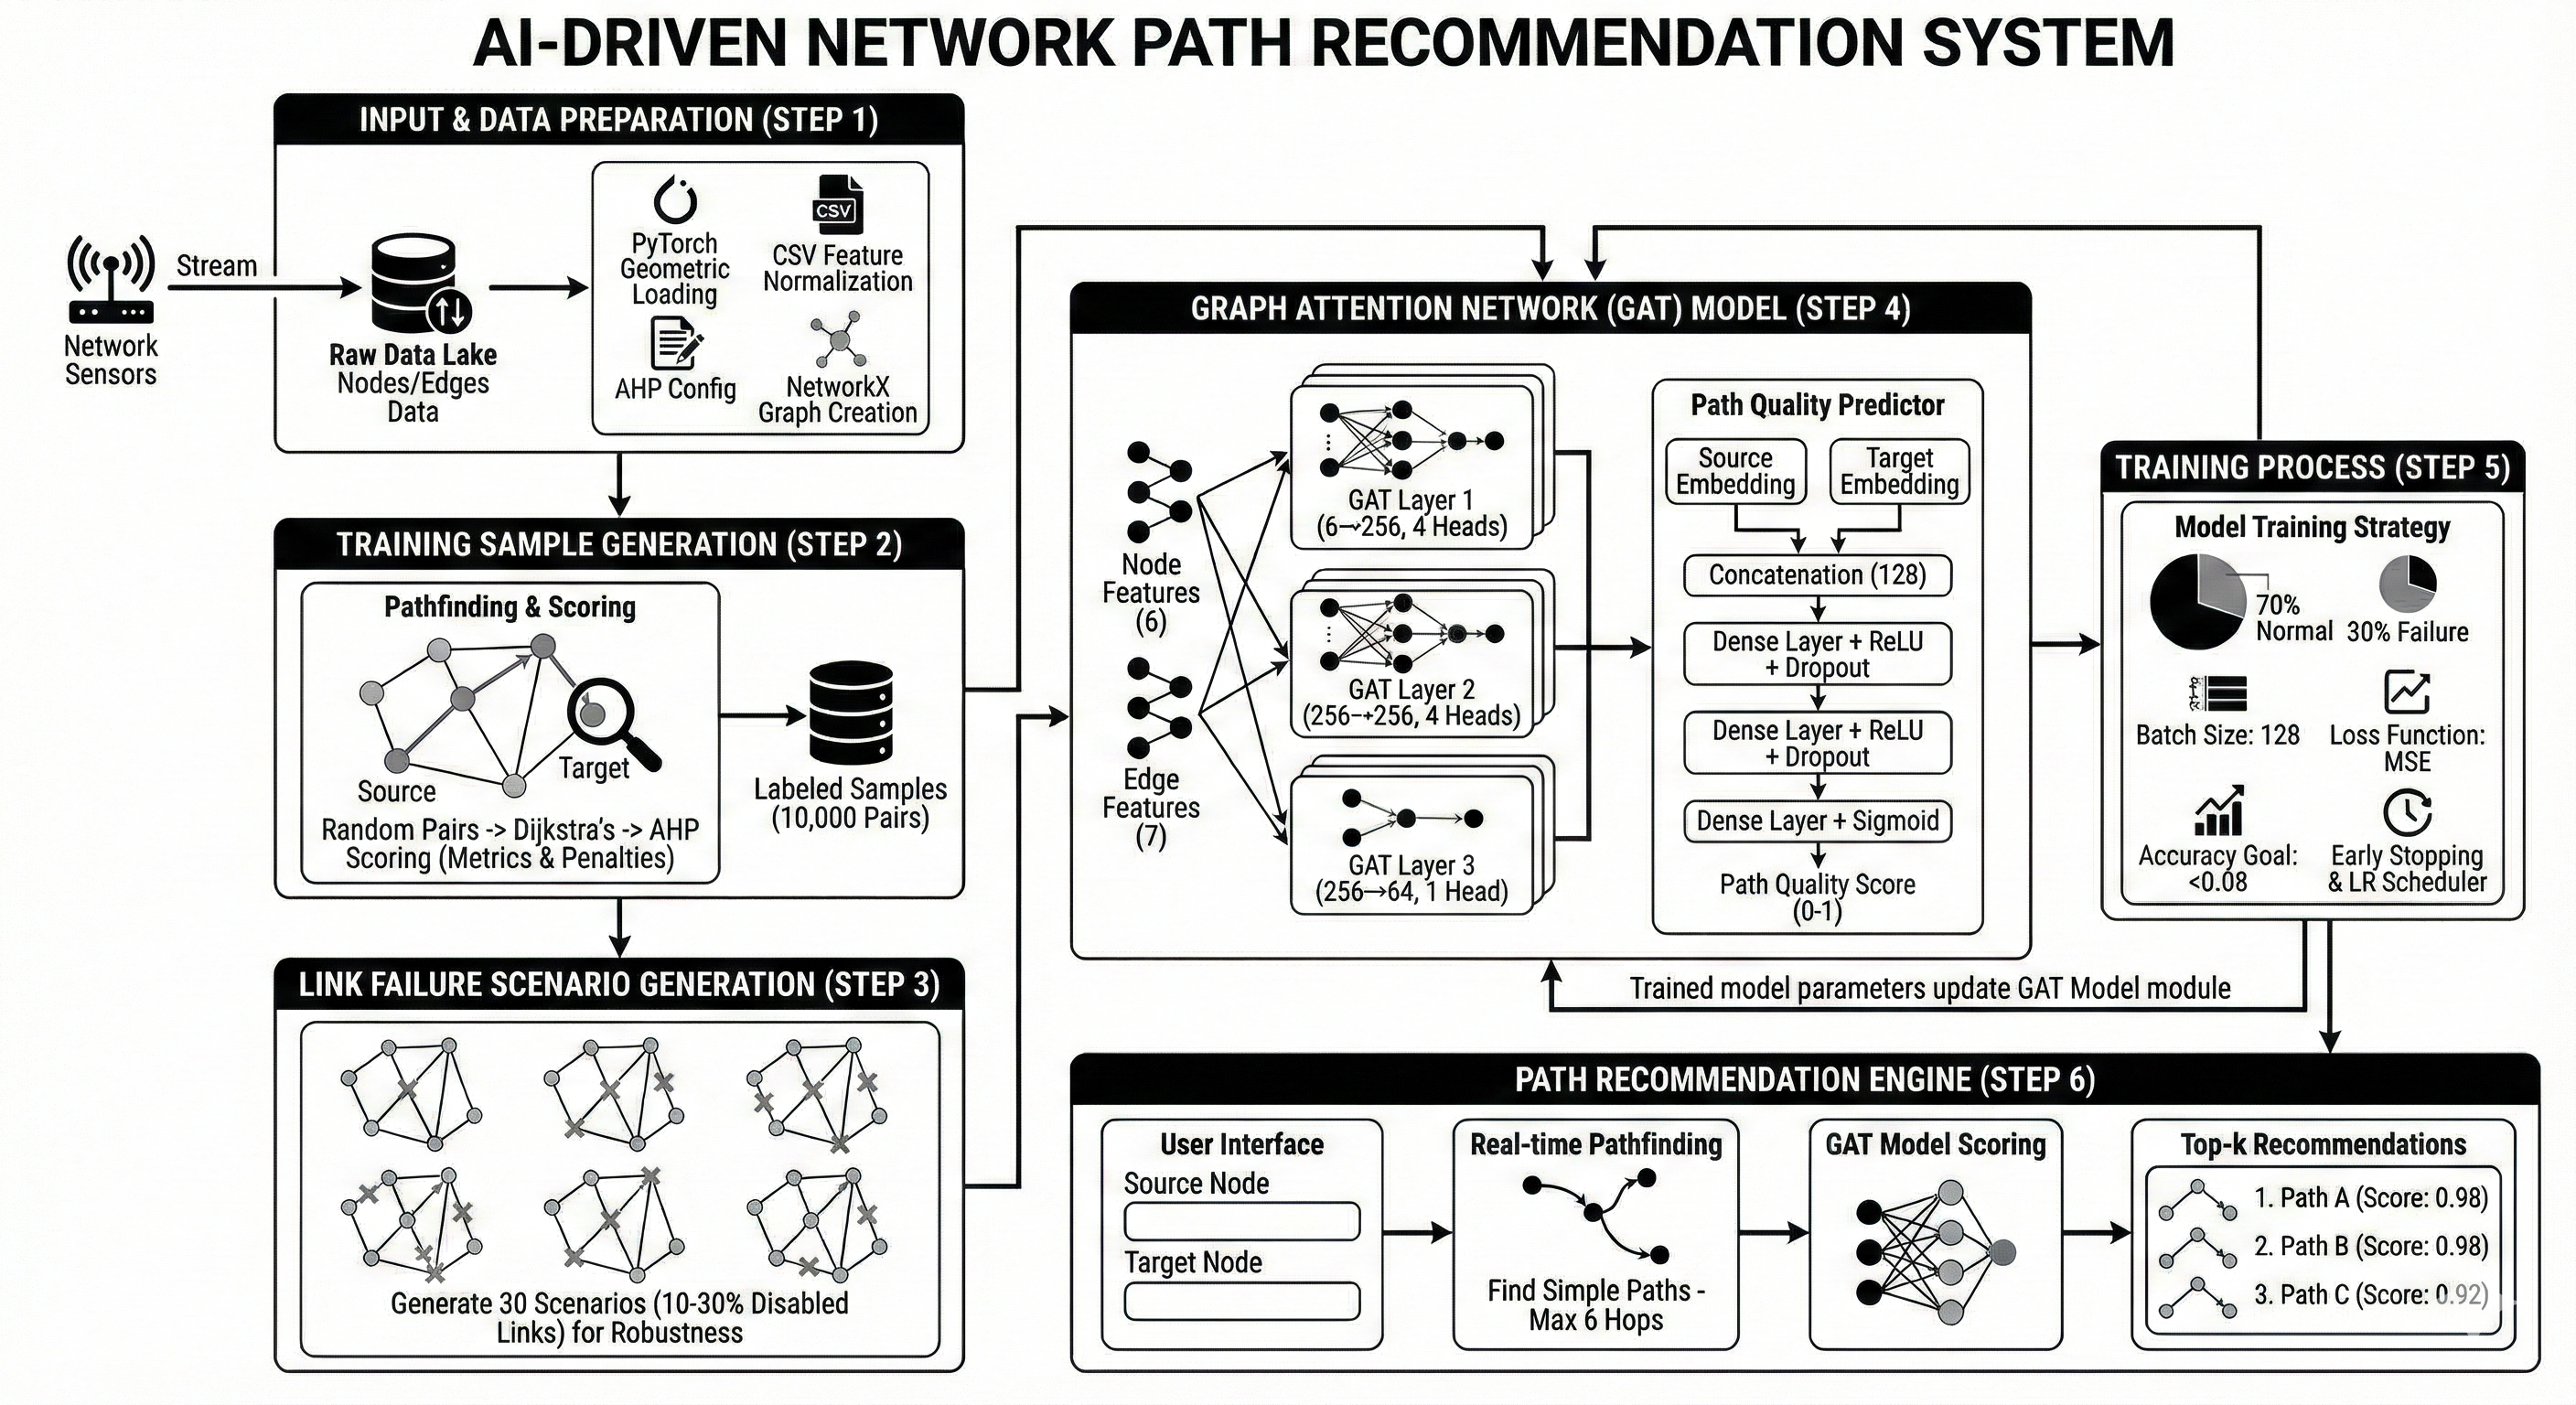
\includegraphics[width=1.0\textwidth]{images/model_flow.png}
    \caption{Alur Pengembangan dan Pelatihan Model GAT}
    \label{fig:model_pipeline}
\end{figure}

\subsubsection{Persiapan Data dan Pelabelan}

Data yang telah dinormalisasi dimuat ke dalam format PyTorch Geometric Data object yang merepresentasikan graf jaringan. Node features direpresentasikan sebagai matrix $\mathbf{X} \in \mathbb{R}^{N \times 6}$ yang berisi 6 fitur untuk setiap node (CPU usage, RAM usage, traffic in, traffic out, interface utilization, status). Edge index direpresentasikan sebagai $\mathbf{E} \in \mathbb{Z}^{2 \times M}$ dalam format adjacency list yang merepresentasikan koneksi antar node. Edge features direpresentasikan sebagai matrix $\mathbf{E}_{\text{attr}} \in \mathbb{R}^{M \times 7}$ yang berisi 7 fitur untuk setiap edge.

Untuk meningkatkan robustness model dalam menghadapi kondisi jaringan yang tidak ideal, dilakukan generasi data sintetis dengan simulasi kegagalan link. Pendekatan ini penting karena dalam operasional nyata, jaringan sering mengalami gangguan parsial. Dari graf topologi original, dibuat 30 skenario kegagalan yang berbeda dimana setiap skenario menonaktifkan 10-30\% edge secara random. Edge yang dinonaktifkan dipilih menggunakan random sampling tanpa replacement, dan setiap skenario disimpan sebagai modified PyTorch Geometric Data object.

Distribusi skenario kegagalan link dibagi menjadi tiga kategori sebagaimana ditunjukkan pada Tabel \ref{tab:failure_scenarios}. Kategori minor failure dengan persentase link disabled 10-15\% sebanyak 10 skenario, moderate failure dengan persentase 15-25\% sebanyak 12 skenario, dan major failure dengan persentase 25-30\% sebanyak 8 skenario.

\begin{table}[H]
    \centering
    \caption{Distribusi Skenario Kegagalan Link}
    \label{tab:failure_scenarios}
    \begin{tabular}{|l|c|c|}
        \hline
        \textbf{Kategori} & \textbf{Persentase Link Disabled} & \textbf{Jumlah Skenario} \\ \hline
        Minor Failure & 10-15\% & 10 \\ \hline
        Moderate Failure & 15-25\% & 12 \\ \hline
        Major Failure & 25-30\% & 8 \\ \hline
    \end{tabular}
\end{table}

Tujuan failure scenarios adalah untuk melatih model agar dapat beradaptasi dengan perubahan topologi, menghindari overfitting pada topologi statis, meningkatkan kemampuan generalisasi model, dan mensimulasikan kondisi real-world dimana link bisa gagal sewaktu-waktu. Selama training, model akan bergantian dilatih menggunakan graf normal untuk belajar routing optimal dan graf dengan failure scenarios untuk belajar failover routing.

\subsubsection{Arsitektur Graph Attention Network (GAT)}

Model yang digunakan dalam penelitian ini adalah Graph Attention Network (GAT), sebuah arsitektur Graph Neural Network yang menggunakan mekanisme attention untuk memberikan bobot berbeda pada tetangga setiap node. Arsitektur ini dipilih karena kemampuannya dalam menangkap struktur graf yang kompleks dan heterogen seperti topologi jaringan komputer.

Model GAT dalam penelitian ini terdiri dari tiga layer GAT dengan konfigurasi yang dirancang secara bertahap. Layer pertama merupakan input layer dengan input dimension 6 (node features), output dimension 64, dan 4 attention heads sehingga total output dimension adalah 256. Layer ini menggunakan edge dimension 7 untuk edge features dalam attention mechanism, activation function ELU (Exponential Linear Unit), dan dropout 0.3. Formula attention untuk layer pertama adalah:
\begin{equation}
\mathbf{h}_i^{(1)} = \Bigg\|_{k=1}^{4} \sigma \left( \sum_{j \in \mathcal{N}(i)} \alpha_{ij}^k \mathbf{W}^k \mathbf{h}_j^{(0)} \right)
\end{equation}
dimana $\alpha_{ij}^k$ adalah attention weight untuk head ke-$k$, $\mathbf{W}^k$ adalah weight matrix, dan $\|$ adalah concatenation operator.

Layer kedua merupakan hidden layer dengan input dimension 256 dari layer pertama, output dimension 64, dan 4 attention heads sehingga total output dimension adalah 256. Layer ini juga menggunakan edge dimension 7, activation function ELU, dan dropout 0.3. Layer ini berfungsi untuk memperdalam representasi dengan menangkap pola interaksi yang lebih kompleks antar node dalam radius 2-hop neighborhood.

Layer ketiga merupakan output layer dengan input dimension 256 dari layer kedua, output dimension 64, dan hanya 1 attention head untuk agregasi final. Layer ini menggunakan edge dimension 7, tidak menggunakan activation function (linear), dan dropout 0.3. Layer final menghasilkan node embeddings dengan dimensi 64 yang merepresentasikan karakteristik setiap node dalam konteks graf.

Setelah GAT layers menghasilkan node embeddings, digunakan Path Quality Predictor berupa feed-forward neural network untuk memprediksi skor kualitas jalur. Input dari predictor adalah concatenation dari embeddings source dan target node untuk setiap hop dengan dimensi total 128 (64 + 64). Hidden layer pertama menggunakan transformasi linear dari 128 ke 128 dengan aktivasi ReLU dan dropout 0.3. Hidden layer kedua menggunakan transformasi linear dari 128 ke 64 dengan aktivasi ReLU dan dropout 0.3. Output layer menggunakan transformasi linear dari 64 ke 1 dengan aktivasi sigmoid, menghasilkan quality score dalam range [0, 1].

Formula prediksi untuk single hop adalah:
\begin{equation}
q_{\text{hop}}(i,j) = \sigma \left( \mathbf{W}_3 \cdot \text{ReLU}\left(\mathbf{W}_2 \cdot \text{ReLU}\left(\mathbf{W}_1 \cdot [\mathbf{h}_i \| \mathbf{h}_j]\right)\right) \right)
\end{equation}
dimana $\sigma$ adalah fungsi sigmoid dan $\|$ menunjukkan operasi concatenation.

Untuk jalur lengkap $P = \{v_1, v_2, \ldots, v_k\}$, skor total dihitung dengan:
\begin{equation}
Q_{\text{path}} = \left( \frac{1}{k-1} \sum_{i=1}^{k-1} q_{\text{hop}}(v_i, v_{i+1}) \right) \times (1 - 0.03 \cdot (k-1))
\end{equation}

Pemilihan hyperparameters didasarkan pada trade-off antara kapasitas model dan computational cost. Hidden dimension 64 cukup untuk menangkap kompleksitas jaringan tanpa overfitting. Multi-head attention dengan 4 heads memungkinkan model belajar berbagai aspek relasi antar node secara paralel seperti proximity, bandwidth similarity, dan load balance. Tiga layers memberikan receptive field 3-hop yang mencukupi untuk jaringan dengan diameter relatif kecil. Dropout 0.3 digunakan sebagai regularisasi untuk mencegah overfitting, terutama penting karena model dilatih dengan data sintetis. Activation function ELU memberikan performa lebih baik dibanding ReLU untuk graph neural networks karena memiliki smooth gradient untuk nilai negatif.

Model memiliki total approximately 500,000 trainable parameters yang terdistribusi sekitar 350,000 parameters pada GAT layers dan 150,000 parameters pada path predictor MLP.

\subsubsection{Strategi Pelatihan Model}

Proses pelatihan model dirancang dengan strategi khusus untuk mengoptimalkan performa pada task path recommendation dalam konteks jaringan yang dinamis. Konfigurasi training menggunakan optimizer Adam dengan initial learning rate 0.001 dan weight decay $5 \times 10^{-4}$. Loss function yang digunakan adalah Mean Squared Error (MSE) dengan batch size 128 samples. Maximum epochs diset 1000 dengan early stopping patience 25 epochs. Gradient clipping diterapkan dengan max norm 1.0, dan pembagian train/validation split adalah 80\% untuk training dan 20\% untuk validation. Pelatihan dilakukan pada CPU Intel i7-1370P.


Model dilatih menggunakan fungsi objektif \textit{Mean Squared Error} (MSE) untuk meminimalkan selisih antara prediksi model dengan label target yang dihasilkan oleh sistem \textit{rule-based}:
\begin{equation}
\mathcal{L}_{\text{MSE}} = \frac{1}{N} \sum_{i=1}^{N} \left(Q_{\text{pred}}^{(i)} - Q_{\text{rule}}^{(i)}\right)^2
\end{equation}
dimana $Q_{\text{pred}}$ adalah skor output dari GAT dan $Q_{\text{rule}}$ adalah skor \textit{ground truth} yang dihitung menggunakan kombinasi bobot AHP dan aturan penalti hop.
MSE dipilih karena karakteristik tugas ini adalah regresi nilai kualitas dalam rentang kontinu [0,1].



Penelitian ini menggunakan Cosine Annealing with Warm Restarts untuk learning rate scheduling dengan formula:
\begin{equation}
\eta_t = \eta_{\min} + \frac{1}{2}(\eta_{\max} - \eta_{\min})\left(1 + \cos\left(\frac{T_{\text{cur}}}{T_i}\pi\right)\right)
\end{equation}
dengan parameter $T_0 = 20$ epochs untuk periode restart pertama, $T_{\text{mult}} = 2$ dimana periode restart dikali 2 setiap restart, dan $\eta_{\min} = 10^{-6}$ sebagai minimum learning rate. Scheduling ini memungkinkan model "escape" dari local minima dengan periodic restart pada learning rate yang lebih tinggi.

Untuk melatih model yang robust terhadap failure, digunakan strategi alternating training dimana model dilatih bergantian menggunakan graf normal (1/31 epochs) dan berbagai kondisi failure (30/31 epochs). Strategi ini memastikan model terpapar dengan kondisi normal untuk belajar routing optimal dan kondisi failure untuk belajar failover routing.

Untuk setiap epoch, training batch terdiri dari 70\% samples dari kondisi normal dan 30\% samples dari kondisi failure. Komposisi ini berdasarkan asumsi bahwa dalam operasional nyata, jaringan mayoritas berada dalam kondisi normal, failure events terjadi secara sporadis, model harus tetap perform optimal pada kondisi normal, dan model harus adaptif ketika failure terjadi.

Untuk mencegah overfitting, diterapkan early stopping dengan monitoring validation loss, patience 25 epochs tanpa improvement, improvement threshold 0.5\% reduction in validation loss atau 1\% increase in validation accuracy, dan best model disimpan berdasarkan validation loss terendah. Gradient clipping diterapkan dengan threshold $\tau = 1.0$ untuk mencegah exploding gradients yang sering terjadi pada graph neural networks.

Validation dilakukan setiap epoch dengan validation set 20\% dari total samples (2,000 samples), evaluasi menggunakan graf normal (bukan failure scenarios), dan metrik yang di-track meliputi validation loss (MSE) dan validation accuracy dengan tolerance $\pm 0.05$, $\pm 0.08$, dan $\pm 0.10$.

\subsection{Integrasi Sistem}

Setelah model terlatih dengan baik, dilakukan integrasi antara backend, ML Engine, dan frontend. Proses ini meliputi deployment model GAT sebagai FastAPI service yang dapat diakses melalui REST API, implementasi API call dari backend ke ML Engine untuk mendapatkan rekomendasi jalur, testing end-to-end system flow untuk memastikan semua komponen bekerja dengan baik, dan performance optimization melalui caching dan async processing.

Proses inferensi mengikuti pipeline yang sistematis dimulai dari input preparation dengan loading current network state dan specify source dan target node. Kemudian dilakukan graph processing untuk convert ke NetworkX graph, filter edge aktif, dan compute shortest path sebagai baseline. Path generation dilakukan dengan enumerate semua jalur menggunakan dynamic cutoff untuk membatasi search space. Quality scoring dilakukan melalui forward pass model untuk mendapatkan node embeddings dan menghitung skor setiap jalur. Terakhir dilakukan ranking \& selection untuk sort berdasarkan skor dan return Top-K jalur terbaik.

Optimasi dilakukan untuk meminimalkan latency dengan model caching saat service startup, vectorized operations untuk batch computation, dynamic cutoff untuk limit search space, dan path sampling dengan maksimum 1000 paths. Target inference time yang ditetapkan adalah kurang dari 500ms untuk typical request.

\subsection{Pengujian dan Evaluasi}

Tahap final mencakup pengujian komprehensif sistem dengan berbagai skenario untuk memvalidasi kemampuan model dalam kondisi real-world. Pengujian dilakukan melalui lima skenario utama untuk mengukur performa sistem dari berbagai aspek.

Normal operation testing bertujuan untuk validasi akurasi rekomendasi pada kondisi optimal. Metode yang digunakan adalah generate 100 random source-target pairs dan mengukur metrik Top-1, Top-3, Top-5 accuracy. Single link failure testing bertujuan untuk uji kemampuan failover path dengan metode disable link kritikal dan request recommendation, kemudian mengukur path validity rate dan quality degradation.

Multiple link failures testing merupakan stress test robustness dengan metode disable 10-20\% edges randomly dan mengukur success rate serta average quality score. High traffic condition testing bertujuan untuk uji penghindaran link congested dengan metode set link utilization lebih dari 80\% dan mengukur average utilization jalur rekomendasi. Real-time performance testing bertujuan untuk validasi latency requirement dengan metode simulate 100 concurrent requests dan mengukur p50, p95, p99 latency, serta throughput.

Metrik evaluasi yang digunakan meliputi metrik akurasi model dan metrik performa sistem. Untuk akurasi model, digunakan Top-K recommendation accuracy yang dihitung dengan formula:
\begin{equation}
\text{Acc}_{\text{top-k}} = \frac{1}{N} \sum_{i=1}^{N} \mathbb{1}\left(\text{recommended}_i \in \text{Top-K\_Expert}_i\right)
\end{equation}
dengan target Top-1 minimal 70\%, Top-3 minimal 90\%, dan Top-5 minimal 95\%.

Root Mean Squared Error (RMSE) dihitung dengan formula:
\begin{equation}
\text{RMSE} = \sqrt{\frac{1}{N} \sum_{i=1}^{N} \left(Q_{\text{pred}}^{(i)} - Q_{\text{true}}^{(i)}\right)^2}
\end{equation}
dengan target RMSE kurang dari 0.08.

Mean Absolute Error (MAE) dihitung dengan formula:
\begin{equation}
\text{MAE} = \frac{1}{N} \sum_{i=1}^{N} \left|Q_{\text{pred}}^{(i)} - Q_{\text{true}}^{(i)}\right|
\end{equation}
dengan target MAE kurang dari 0.06.

Untuk metrik performa sistem, diukur inference latency dengan target p95 kurang dari 500ms, throughput dengan target lebih dari 20 request per second, memory usage dengan peak memory kurang dari 500 MB, dan path validity rate yang harus mencapai 100\% (mandatory).

Metode validasi yang digunakan adalah K-Fold cross validation dimana dataset dibagi menjadi 5 folds untuk memastikan generalisasi model. Performa model juga dibandingkan dengan baseline methods seperti shortest path (hop count), Dijkstra with bandwidth only, AHP-Dijkstra (expert system), dan random path selection.

Ablation study dilakukan untuk memahami kontribusi setiap komponen model dengan membandingkan full model yang menggunakan attention, edge features, dan hop penalty dengan variant tanpa attention, variant tanpa edge features, dan variant tanpa hop penalty sebagaimana ditunjukkan pada Tabel \ref{tab:ablation}.
\begin{table}[H]
    \centering
    \caption{Ablation Study Variants}
    \label{tab:ablation}
    \begin{tabular}{|l|c|c|c|}
        \hline
        \textbf{Model Variant} & \textbf{Attention} & \textbf{Edge Features} & \textbf{Hop Penalty} \\ \hline
        Full Model & \checkmark & \checkmark & \checkmark \\ \hline
        Without Attention & $\times$ & \checkmark & \checkmark \\ \hline
        Without Edge Features & \checkmark & $\times$ & \checkmark \\ \hline
        Without Hop Penalty & \checkmark & \checkmark & $\times$ \\ \hline
    \end{tabular}
\end{table}

Kriteria keberhasilan penelitian ditetapkan berdasarkan target metrik yang telah ditentukan sebagaimana ditunjukkan pada Tabel \ref{tab:success_criteria}. Top-3 accuracy harus mencapai minimal 90\%, RMSE kurang dari 0.08, inference latency (p95) kurang dari 500ms, path validity rate harus 100\%, dan improvement over shortest path minimal 15\%.

\begin{table}[H]
    \centering
    \caption{Kriteria Keberhasilan Penelitian}
    \label{tab:success_criteria}
    \begin{tabular}{|l|c|l|}
        \hline
        \textbf{Metrik} & \textbf{Target} & \textbf{Status} \\ \hline
        Top-3 Accuracy & $\geq 90\%$ & [To be measured] \\ \hline
        RMSE & $< 0.08$ & [To be measured] \\ \hline
        Inference Latency (p95) & $< 500$ms & [To be measured] \\ \hline
        Path Validity Rate & 100\% & [To be measured] \\ \hline
        Improvement over Shortest Path & $\geq 15\%$ & [To be measured] \\ \hline
    \end{tabular}
\end{table}

\subsection{Contoh Perhitungan Numerik Pelabelan Data}

Untuk memperjelas mekanisme \textit{Rule-Based Labeling} yang digunakan dalam menghasilkan \textit{Ground Truth} ($Q_{path}$), berikut disajikan simulasi perhitungan pada sebuah jalur sederhana. Demi penyederhanaan, perhitungan ini hanya menggunakan sampel 2 fitur node dan 2 fitur edge.

\paragraph{Skenario Jalur}
Misalkan terdapat sebuah jalur $P$ dari Node A ke Node C yang melalui Node B ($A \rightarrow B \rightarrow C$).
\begin{itemize}
    \item Jumlah Node ($k$) = 3 (A, B, C)
    \item Jumlah Hop ($h$) = 2
    \item Konstanta penalti hop ($\alpha$) = 0.05
\end{itemize}

\paragraph{1. Data Mentah dan Normalisasi}
Asumsikan data mentah hasil monitoring SNMP dan proses normalisasi (\textit{Min-Max Scaling}) adalah sebagai berikut:

\textbf{a. Sampel Fitur Node (CPU \& RAM):}
\begin{table}[H]
    \centering
    \small
    \caption{Sampel Data Normalisasi Node}
    \label{tab:sample_node_norm}
    \begin{tabular}{|c|c|c|c|c|}
        \hline
        \textbf{Node} & \textbf{Metric} & \textbf{Nilai Mentah} & \textbf{Range Min-Max} & \textbf{Nilai Norm ($f_i$)} \\ \hline
        \multirow{2}{*}{Node B} & CPU Usage & 60\% & 0 - 100\% & 0.60 \\ \cline{2-5}
         & RAM Usage & 40\% & 0 - 100\% & 0.40 \\ \hline
    \end{tabular}
\end{table}
\noindent \textit{Catatan: Node A dan Node C diasumsikan memiliki nilai skor akhir yang sama dengan Node B untuk penyederhanaan contoh.}

\textbf{b. Sampel Fitur Edge (Bandwidth \& Distance):}
\begin{table}[H]
    \centering
    \small
    \caption{Sampel Data Normalisasi Edge}
    \label{tab:sample_edge_norm}
    \begin{tabular}{|c|c|c|c|c|}
        \hline
        \textbf{Edge} & \textbf{Metric} & \textbf{Nilai Mentah} & \textbf{Range Min-Max} & \textbf{Skor ($s_k$)} \\ \hline
        \multirow{2}{*}{$A \rightarrow B$} & BW Util & 80\% & 0 - 100\% & $1 - 0.8 = 0.20$ \\ \cline{2-5}
         & Distance & 5 km & 0 - 20 km & $1 - \frac{5}{20} = 0.75$ \\ \hline
        \multirow{2}{*}{$B \rightarrow C$} & BW Util & 20\% & 0 - 100\% & $1 - 0.2 = 0.80$ \\ \cline{2-5}
         & Distance & 2 km & 0 - 20 km & $1 - \frac{2}{20} = 0.90$ \\ \hline
    \end{tabular}
\end{table}
\noindent \textit{Catatan: Nilai dinormalisasi menjadi "Higher is Better". Untuk metrik "Lower is Better" (seperti Utilisasi dan Jarak), skor dihitung sebagai $(1 - \text{nilai norm})$.}

\paragraph{2. Penerapan Bobot AHP}
Misalkan berdasarkan kuesioner pakar, diperoleh bobot prioritas relatif (disederhanakan) sebagai berikut:
\begin{itemize}
    \item \textbf{Bobot Node:} $w_{CPU} = 0.6$, $w_{RAM} = 0.4$
    \item \textbf{Bobot Edge:} $w_{BW} = 0.7$, $w_{Dist} = 0.3$
\end{itemize}

\paragraph{3. Perhitungan Skor Komponen}

\begin{itemize}
    \item[\textbf{a.}] \textbf{Skor Kualitas Node ($Q_{node}$)} \\
    Menggunakan Persamaan (3.4), skor kualitas intrinsik Node B dihitung (ingat: semakin rendah load, semakin baik skornya, maka digunakan $1-f_i$):
    \begin{align*}
        Q_{node}(B) &= (1 - f_{CPU}) \cdot w_{CPU} + (1 - f_{RAM}) \cdot w_{RAM} \\
        &= (1 - 0.60) \cdot 0.6 + (1 - 0.40) \cdot 0.4 \\
        &= (0.40 \cdot 0.6) + (0.60 \cdot 0.4) \\
        &= 0.24 + 0.24 \\
        &= \mathbf{0.48}
    \end{align*}

    \item[\textbf{b.}] \textbf{Skor Kualitas Edge ($Q_{edge}$)} \\
    Menggunakan Persamaan (3.3):

    \vspace{0.2cm} % Memberi sedikit jarak
    \textit{Untuk Edge $A \rightarrow B$ (Kualitas Buruk pada Bandwidth):}
    \begin{align*}
        Q_{edge}(A \rightarrow B) &= s_{BW} \cdot w_{BW} + s_{Dist} \cdot w_{Dist} \\
        &= 0.20 \cdot 0.7 + 0.75 \cdot 0.3 \\
        &= 0.14 + 0.225 \\
        &= \mathbf{0.365}
    \end{align*}

    \textit{Untuk Edge $B \rightarrow C$ (Kualitas Baik):}
    \begin{align*}
        Q_{edge}(B \rightarrow C) &= s_{BW} \cdot w_{BW} + s_{Dist} \cdot w_{Dist} \\
        &= 0.80 \cdot 0.7 + 0.90 \cdot 0.3 \\
        &= 0.56 + 0.27 \\
        &= \mathbf{0.830}
    \end{align*}
\end{itemize}

\paragraph{4. Perhitungan Label Akhir Jalur ($Q_{path}$)}
Menggunakan Persamaan (3.5), rata-rata skor seluruh komponen dihitung dan kemudian diterapkan penalti hop.

Komponen jalur terdiri dari 3 Node (A, B, C) dan 2 Edge ($A \rightarrow B$, $B \rightarrow C$).
Asumsi $Q_{node}(A) = 0.48$ dan $Q_{node}(C) = 0.48$ (sama dengan B).

\begin{align*}
    \text{Sum Component} &= Q_{node}(A) + Q_{node}(B) + Q_{node}(C) + Q_{edge}(AB) + Q_{edge}(BC) \\
    &= 0.48 + 0.48 + 0.48 + 0.365 + 0.830 \\
    &= 2.635
\end{align*}

Jumlah komponen ($2k - 1$) = $2(3) - 1 = 5$.

\begin{align*}
    Q_{path} &= \left( \frac{2.635}{5} \right) \times (1 - 0.05 \cdot (3-1)) \\
    &= 0.527 \times (1 - 0.1) \\
    &= 0.527 \times 0.9 \\
    &= \mathbf{0.4743}
\end{align*}

\textbf{Interpretasi:}
Nilai $Q_{path} = 0.4743$ (Skala 0-1) menunjukkan bahwa jalur ini memiliki kualitas \textbf{Fair/Cukup}. Meskipun Edge $B \rightarrow C$ sangat bagus, skor jatuh signifikan karena Edge $A \rightarrow B$ mengalami kongesti berat (BW Util 80\%) dan beban CPU Node B yang agak tinggi. Nilai inilah yang akan menjadi \textit{Target Label} ($y$) bagi model GAT saat proses training.

\subsection{Contoh Perhitungan Numerik GAT}

Untuk memberikan pemahaman yang lebih konkret tentang mekanisme GAT, berikut disajikan contoh perhitungan numerik lengkap. Contoh ini menggunakan topologi sederhana yang merepresentasikan segmen jaringan dengan 3 node yang saling terhubung (fully connected).

\paragraph{Representasi Visual Topologi dan Fitur}
Graf jaringan $\mathcal{G}$ terdiri dari 3 node: Node A (Core), serta Node B dan Node C (Distribution). Setiap node memiliki vektor fitur awal $\vec{h}_i$ berdimensi $F=2$ yang merepresentasikan [CPU Usage, Bandwidth Util].

\begin{figure}[H]
    \centering
    \begin{tikzpicture}[
        node_style/.style={circle, draw=black, thick, fill=blue!10, minimum size=1.2cm, font=\bfseries},
        edge_style/.style={thick, -},
        feature_style/.style={rectangle, draw=gray, dashed, fill=white, font=\small, align=center, inner sep=4pt}
    ]

        % 1. Definisi Node (Posisi Segitiga)
        \node[node_style] (A) at (0, 2) {A};
        \node[node_style] (B) at (-2.5, -1) {B};
        \node[node_style] (C) at (2.5, -1) {C};

        % 2. Menggambar Koneksi (Edge)
        \draw[edge_style] (A) -- (B);
        \draw[edge_style] (A) -- (C);
        \draw[edge_style] (B) -- (C);

        % 3. Menambahkan Label Fitur di dekat Node
        % Fitur Node A
        \node[feature_style, right=0.3cm of A] (featA) {
            $\vec{h}_A = \begin{bmatrix} 0.3 \\ 0.5 \end{bmatrix}$ \\
            \scriptsize{(CPU: 30\%, BW: 50\%)}
        };

        % Fitur Node B
        \node[feature_style, below=0.3cm of B] (featB) {
            $\vec{h}_B = \begin{bmatrix} 0.7 \\ 0.4 \end{bmatrix}$ \\
            \scriptsize{(CPU: 70\%, BW: 40\%)}
        };

        % Fitur Node C
        \node[feature_style, below=0.3cm of C] (featC) {
            $\vec{h}_C = \begin{bmatrix} 0.5 \\ 0.2 \end{bmatrix}$ \\
            \scriptsize{(CPU: 50\%, BW: 20\%)}
        };

        % Garis bantu tipis dari node ke kotak fitur (opsional, agar rapi)
        \draw[gray, dotted] (A) -- (featA);
        \draw[gray, dotted] (B) -- (featB);
        \draw[gray, dotted] (C) -- (featC);

    \end{tikzpicture}
    \caption{Visualisasi Topologi Contoh dan Vektor Fitur Input Node}
    \label{fig:gat_example_topology}
\end{figure}

Berdasarkan visualisasi pada Gambar \ref{fig:gat_example_topology}, matriks adjacency ($\mathbf{A}$) untuk topologi tersebut adalah:
\begin{equation}
    \mathbf{A} = \begin{bmatrix}
    1 & 1 & 1 \\
    1 & 1 & 1 \\
    1 & 1 & 1
    \end{bmatrix}
\end{equation}
(Nilai 1 menunjukkan adanya koneksi langsung, termasuk \textit{self-loop} pada diagonal utama).

\paragraph{Parameter Model}
Untuk kesederhanaan, gunakan \textit{single attention head} ($K=1$) dengan dimensi output $F' = 2$. Parameter yang dipelajari adalah:

\begin{equation}
    \mathbf{W} = \begin{bmatrix}
    1.0 & 0.5 \\
    0.5 & 1.0
    \end{bmatrix}, \quad
    \vec{a} = \begin{bmatrix}
    0.5 \\
    0.5 \\
    0.3 \\
    0.3
    \end{bmatrix}
\end{equation}

dimana $\mathbf{W}$ adalah matriks transformasi linear ($2 \times 2$) dan $\vec{a}$ adalah vektor parameter atensi ($4 \times 1$, untuk concatenation 2 node).

\paragraph{Tahap 1: Transformasi Linear}
Hitung fitur hasil transformasi ($\vec{z}_i = \mathbf{W}\vec{h}_i$) untuk setiap node:

\begin{align*}
    \vec{z}_A &= \begin{bmatrix} 1.0 & 0.5 \\ 0.5 & 1.0 \end{bmatrix} \begin{bmatrix} 0.3 \\ 0.5 \end{bmatrix} = \begin{bmatrix} 0.55 \\ 0.65 \end{bmatrix} \\
    \vec{z}_B &= \begin{bmatrix} 1.0 & 0.5 \\ 0.5 & 1.0 \end{bmatrix} \begin{bmatrix} 0.7 \\ 0.4 \end{bmatrix} = \begin{bmatrix} 0.90 \\ 0.75 \end{bmatrix} \\
    \vec{z}_C &= \begin{bmatrix} 1.0 & 0.5 \\ 0.5 & 1.0 \end{bmatrix} \begin{bmatrix} 0.5 \\ 0.2 \end{bmatrix} = \begin{bmatrix} 0.60 \\ 0.45 \end{bmatrix}
\end{align*}

\paragraph{Tahap 2: Komputasi Skor Atensi Mentah}
Kita fokus menghitung update untuk \textbf{Node A}. Hitung skor atensi terhadap dirinya sendiri dan tetangganya (B dan C). Gunakan $\text{LeakyReLU}$ dengan slope negatif 0.2. Rumus: $e_{ij} = \text{LeakyReLU}(\vec{a}^T [\vec{z}_i \| \vec{z}_j])$.

\textbf{1. Skor atensi A terhadap A (self-attention):}
Concatenation $[\vec{z}_A \| \vec{z}_A] = [0.55, 0.65, 0.55, 0.65]^T$.
\begin{align*}
    e_{AA} &= \text{LeakyReLU}(\vec{a} \cdot [0.55, 0.65, 0.55, 0.65]^T) \\
    &= \text{LeakyReLU}(0.5(0.55) + 0.5(0.65) + 0.3(0.55) + 0.3(0.65)) \\
    &= \text{LeakyReLU}(0.275 + 0.325 + 0.165 + 0.195) \\
    &= \text{LeakyReLU}(0.96) = \mathbf{0.96}
\end{align*}

\textbf{2. Skor atensi A terhadap B:}
Concatenation $[\vec{z}_A \| \vec{z}_B] = [0.55, 0.65, 0.90, 0.75]^T$.
\begin{align*}
    e_{AB} &= \text{LeakyReLU}(0.5(0.55) + 0.5(0.65) + 0.3(0.90) + 0.3(0.75)) \\
    &= \text{LeakyReLU}(0.6 + 0.27 + 0.225) \\
    &= \text{LeakyReLU}(1.095) = \mathbf{1.095}
\end{align*}

\textbf{3. Skor atensi A terhadap C:}
Concatenation $[\vec{z}_A \| \vec{z}_C] = [0.55, 0.65, 0.60, 0.45]^T$.
\begin{align*}
    e_{AC} &= \text{LeakyReLU}(0.5(0.55) + 0.5(0.65) + 0.3(0.60) + 0.3(0.45)) \\
    &= \text{LeakyReLU}(0.6 + 0.18 + 0.135) \\
    &= \text{LeakyReLU}(0.915) = \mathbf{0.915}
\end{align*}

\paragraph{Tahap 3: Normalisasi Softmax}
Hitung koefisien atensi $\alpha_{ij}$ menggunakan Softmax:
$$ \sum \exp(e) = \exp(0.96) + \exp(1.095) + \exp(0.915) \approx 2.61 + 2.99 + 2.50 = 8.10 $$

\begin{itemize}
    \item $\alpha_{AA} = \frac{2.61}{8.10} = \mathbf{0.32}$ (Atensi ke diri sendiri)
    \item $\alpha_{AB} = \frac{2.99}{8.10} = \mathbf{0.37}$ (Atensi ke Node B - Prioritas Tertinggi)
    \item $\alpha_{AC} = \frac{2.50}{8.10} = \mathbf{0.31}$ (Atensi ke Node C)
\end{itemize}

\textit{Interpretasi:} Model memberikan bobot terbesar (37\%) ke Node B karena fitur-fiturnya menghasilkan skor atensi tertinggi.

\paragraph{Tahap 4: Agregasi Fitur}
Hitung fitur baru Node A ($\vec{h}'_A$) sebagai kombinasi linear terbobot, lalu terapkan aktivasi (misal ReLU).

\begin{align*}
    \vec{h}'_A &= \sigma ( \alpha_{AA}\vec{z}_A + \alpha_{AB}\vec{z}_B + \alpha_{AC}\vec{z}_C ) \\
    &= \sigma \left( 0.32 \begin{bmatrix} 0.55 \\ 0.65 \end{bmatrix} + 0.37 \begin{bmatrix} 0.90 \\ 0.75 \end{bmatrix} + 0.31 \begin{bmatrix} 0.60 \\ 0.45 \end{bmatrix} \right) \\
    &= \sigma \left( \begin{bmatrix} 0.176 \\ 0.208 \end{bmatrix} + \begin{bmatrix} 0.333 \\ 0.277 \end{bmatrix} + \begin{bmatrix} 0.186 \\ 0.139 \end{bmatrix} \right) \\
    &= \sigma \begin{bmatrix} 0.695 \\ 0.624 \end{bmatrix} = \begin{bmatrix} \mathbf{0.695} \\ \mathbf{0.624} \end{bmatrix}
\end{align*}

\textbf{Kesimpulan:} Fitur Node A telah diperbarui dari $[0.3, 0.5]$ menjadi $[0.695, 0.624]$. Nilai baru ini mengandung informasi agregat dari tetangganya, dengan penekanan lebih pada Node B yang dianggap lebih penting oleh mekanisme atensi.
